% Chapter Template

\chapter{Low magnetic field effects in Si:P qubits} % Main chapter title

\label{Chapter6} 

\noindent\hrulefill
\vspace{0.5cm} %\hspace{2cm}
%\small
\begin{flushright}
        ``\emph{In physics, you don't have to go around making trouble for yourself - nature does it for you.}"
\\ 
--Frank Wilczek \\
\end{flushright}

\vspace{0.5cm}


\noindent\hrulefill
\vspace{0.5cm} %\hspace{2cm}
\\
%\small
\hangindent=4cm
%\noindent
\\
Understanding our qubits fully is of utmost importance for large scale quantum computing. In this chapter we analyse the electron spin relaxation the donor electron qubit with external magnetic field and donor confinement depth. We observe interesting effects such as evanescent wave Johnson noise, strain and tunnelling that all influence the relaxation time. These findings give greater insight into the microscopic picture of qubit environment and allows for engineering qubits with improved relaxation times.  
\\ \\
\scriptsize
\hangindent=4cm
The work presented in this chapter has been submitted for publishing in Physical Review B and published in:\\
\textbf{S. Tenberg}, S. Asaad, M. Madzik, M. Johnson, A. Laucht, F. Hudson, D. Jamieson, J. McCallum, A. Dzurak, R. Joynt, A. Morello. ``Electron spin relaxation effects of a single phosphorus donor in silicon at low temperatures.'' \textit{arxiv} (2018).\\
\\
\footnotesize
\hangindent=4cm
\textbf{The author acknowledges S. Asaad for assistance with the measurement software and the $T_1$ measurements,  M. Madzik for the $T_1$ measurement of device 2018A in figure \ref{fig:magnetic field dependence} and R. Joynt for the EWJN theory.}\\

%\vspace{0.5cm}

\noindent \hrulefill
\clearpage

\normalsize

\section{\label{sec:introduction}Introduction}

The electron spin-lattice relaxation time $T_1$ in donors in silicon is of great interest. Not only gives it insight into the fundamental physics of the system but also is extremely relevant for donor spin qubits which have proven to be excellent candidates for quantum computation \cite{Muhonen2014, Muhonen2015}. Indeed the qubit coherence times of up to $T_2=1\,$s approach the limit set by the relaxation time \cite{Kalra2016}. However, few experiments have been performed to learn more about the mechanisms limiting $T_1$. 

Generally, relaxation happens due to fluctuations in the transverse elements of the Hamiltonian at the Larmor frequency of the spin states. This requires the spin to be coupled to a phonon reservoir.
As silicon is not a piezoelectric material this coupling is only achieved by the deformation potential. Phonons, in form of acoustic waves, deform the lattice while travelling through the crystal. This breaks crystal cubic symmetry which in turn lifts the degeneracy of the six conduction band minima, called valleys. The magnitude of this energy shift is defined by the deformation potential. The relative valley population changes, causing a shift in the g-factor. This shift oscillates with the phonon frequency and relaxes the spin \cite{Hasegawa1960}. Furthermore, local strain couples the $\Gamma$ and $\Delta$ energy bands in one valley, effectively changing the g factor locally, thus also relaxing the spin in the same fashion \cite{Roth1960}. 
This spin-lattice relaxation is described by 
\begin{eqnarray}\label{eq:fullT1}
T_1^{-1} & = & \frac{1}{90\pi}\left(\frac{g_{||}-g_\perp}{g_0}\right)\left(\frac{\Xi_u}{E_{12}}\right)^2\\
& &\left(\frac{1}{\rho \bar{v}_t^5}+\frac{2}{3\rho\bar{v}_l^5}\right)\left(\frac{g_0\mu_0B}{\hbar}\right)^4f(\theta)\cdot k_{\rm B} T
\end{eqnarray}
in the high temperature limit where $\frac{g_{||}-g_\perp}{g_0}$ is the anisotropy in the g-factor, $\Xi_u$ is the deformation potential, $E_{12}$ is the valley orbit splitting between the ground and first excited state, $v_l, v_t$ are the sounds velocities in silicon, $\rho$ is the density of silicon and $f(\theta)$ is an angular factor with regard of the external magnetic field $B_0$ and the crystal axis \cite{Wilson1961}.
At low temperatures ($k_{\rm B}\ll E_z=g_0\mu_0 B$) only spontaneous phonon emission is possible so that $T_1\sim B^5$ is expected \cite{Morello2010, Zwanenburg2013}. 

Previously the dependence of $T_1$ on external magnetic field at low temperatures of donors in silicon has been measured by Morello \textit{et. al.} \cite{Morello2010} on two single phosphorus donors in a CMOS style device and Watson \textit{et. al} \cite{Watson2015} on a single phosphorus donor in a STM hydrogen lithography device. While two of these three measurements conform with each other and follow the expected $T_1\sim B^5$, one measurement by Morello \textit{et. al.} shows a strong deviation. Not only is the magnitude of the $B^5$ relaxation one order of magnitude different but also deviates the measurement from $T_1\sim B^5$ to $T_1\sim B$ at low magnetic fields $B<2\,$T.  

In this paper we present detailed measurements of the relaxation with magnetic field in both enriched silicon $^{28}$Si and natural silicon. We find large deviations in behaviour between different samples which implies a strong dependence of the relaxation on the donor environment. We see a clear $T_1\sim B$ at low magnetic fields for most samples. This dependence seems to be caused by Evanescent wave Johnson noise (EWJN). The magnitude of the $B^5$ relaxation varies by two orders of magnitude between the measured samples. The cause for this effect remains uncertain, though it could be caused by a different concentration of Si29 nuclei or strain variations. Further investigation is necessary. 

Moreover, as the relaxation time approaches multiple seconds, we observe effects of the electro-statical environment on the relaxation. Thus, we study the relaxation with both donor confinement depth (plunge voltage) and the electron number on a nearby single electron transistor (SET). We observe direct tunnelling into the nearby SET electron reservoir reducing the relaxation time for shallow plunging. Once this first-order process is suppressed, second-order tunnelling limits the relaxation time until all tunnelling processes are suppressed at deep plunge voltages $V_p\gg E_z$.

%This study revealed three different effects that influence the relaxation time in this system:  Firstly, we observe an effect that leads to a dominant . 
% EWJN relaxes the donor electron by stimulated emission into the enhanced density of states of the electromagnetic waves decaying from the Aluminium structures on top of the donor.
% Secondly, strain strongly suppresses the phonon relaxation. Lastly, co tunnelling decreases the $T_1$ if the donor is not plunged deep enough below the Fermi level.
 % The $\ket{\uparrow}$ electron escapes from the donor through a virtual co-tunnelling process into free states of the reservoir of the SET island and is replaces by $\ket{\downarrow}$. The tunnel rate strongly depends on the depth of the donor level beneath the Fermi level. Thus it can be mitigated by pulsing deeply below the Fermi level during operation.

The remainder of this paper will elaborate on these findings and is organised as follows. Section \ref{sec:background} presents our physical system and the experimental set up as well as the measurement techniques used to acquire the data. Then section \ref{sec:extB} shows the results of the magnetic field dependence measurements where we both analyse the low magnetic field behaviour in section \ref{sec:ewjn} and the high magnetic field behaviour in section \ref{sec:strain}. Lastly, section \ref{sec:cotunnelling} presents the electrostatic environment measurements. Finally, section \ref{sec:conclusion} discusses the results, open questions and possible future measurements. 


\section{\label{sec:background} The qubit system and measurement methods}

\begin{figure}
\centering
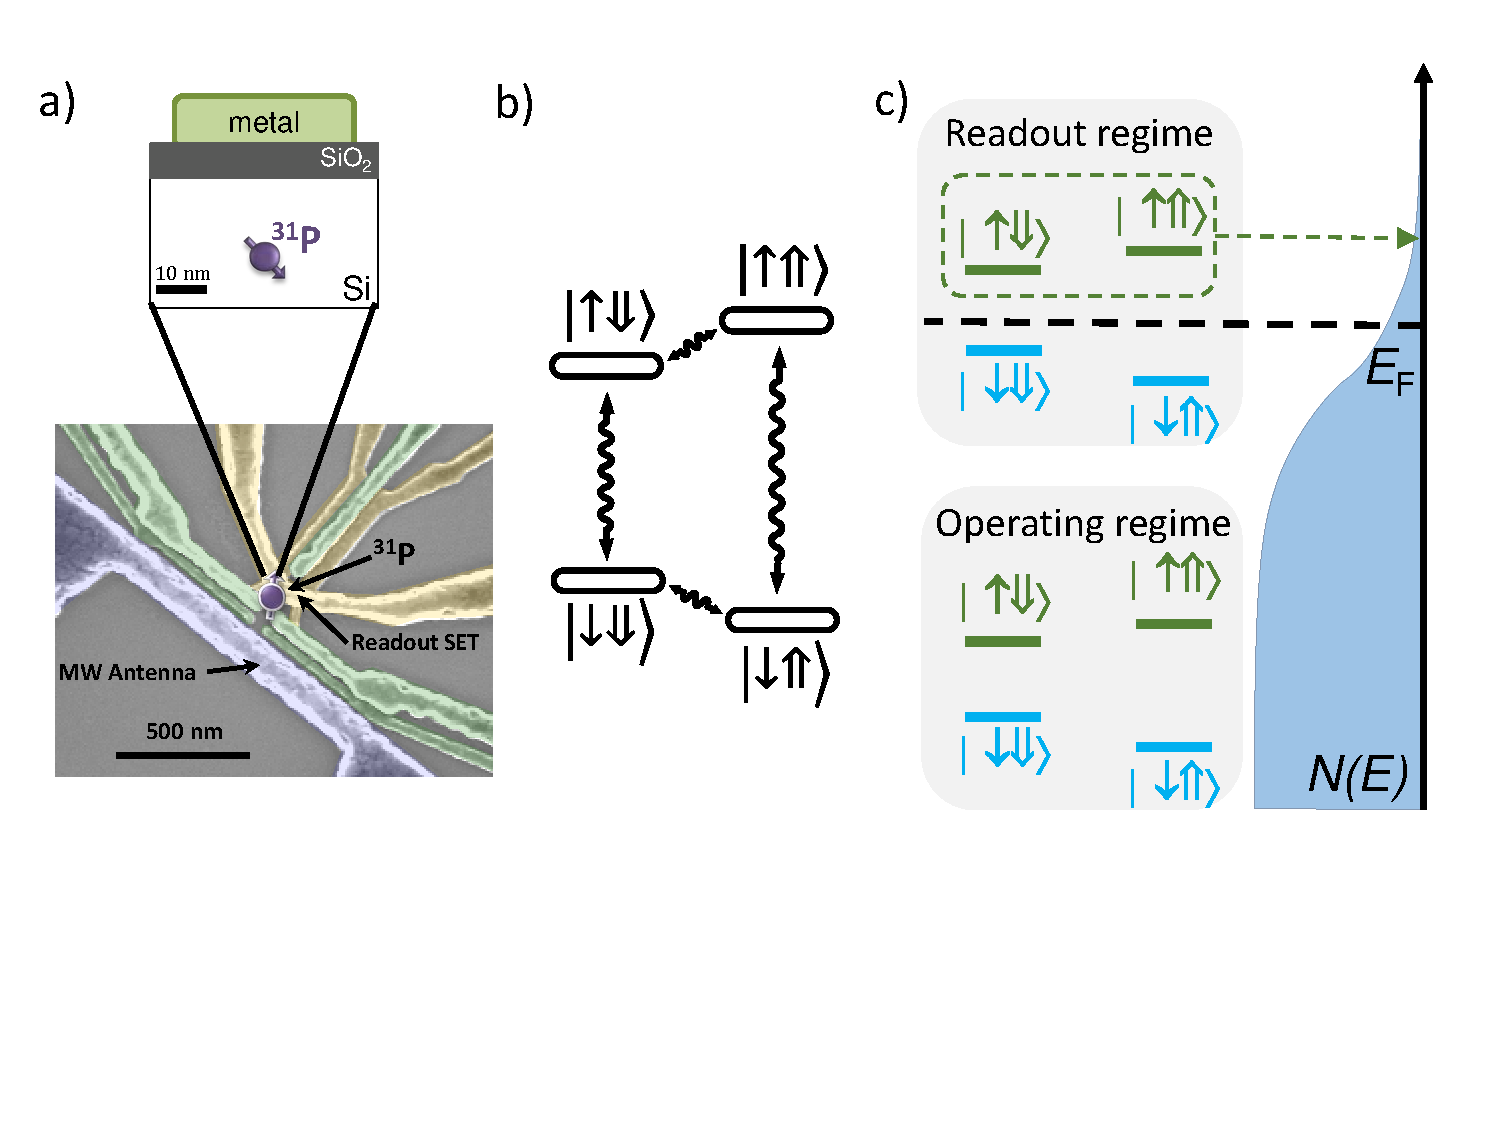
\includegraphics[width=\columnwidth]{figures/fig1.pdf}
\caption{
(a) Schematic of a phosphorus donor implanted in enriched $^{28}$Si with a scanning electron micrograph of an identical device to the one measured. Four gates control the donor potential while a single electron transistor (SET) detects electron tunnel events in its environment to determine the qubit state. A broadband microwave antenna provides an electromagnetic drive for both the electron and the nucleus. b) Energy diagram of the electron-nuclear spin system, with ESR and NMR transitions indicated. (c) Schematic of the two regimes the donor qubit is operated in for the relaxation measurements: 1. Readout regime, where the donor is tuned such that the Fermi level of the SET reservoir lies below $\ket{\uparrow}$ and the electron can tunnel out, producing a current spike, while $\ket{\downarrow}$ lies above and stays confined, keeping the current low. 2. Operating regime, where both spin states are well confined below the Fermi level.
}
\label{fig:device}
\end{figure}

Our qubit is a single electron spin confined by a phosphorus $^{31}$P donor implanted in enriched $^{28}$Si as shown in the schematic in figure \ref{fig:device} (a). An external magnetic field is applied to separate the spin states into a well defined two level system. This leads to a two-qubit system: The donor electron with $S=1/2$ and basis states $\ket{\uparrow},\ket{\downarrow}$ and the $^{31}$P nucleus with $I=1/2$ and basis states $\ket{\Uparrow},\ket{\Downarrow}$. The energy levels of this system are displayed in figure \ref{fig:device} (b). A scanning electron micrograph of the device is shown in figure \ref{fig:device} (a).  Aluminium gates on top of the donor control the electrostatic environment and are used to apply DC pulses while a broadband microwave antenna is used for microwave and radio frequency pulses, allowing for full control over the qubit states. A nearby SET with an electron reservoir of an electron temperature of $T\approx 100\,$mK acts as a readout mechanism for the electron spin state. Therefore, we tune the electrochemical potential of the SET $\mu_{\rm SET}$ and the donor $\mu_d$ such that the donor electron tunnels to the SET reservoir if in state $\ket{\uparrow}$, causing a SET current spike, but stays confined if $\ket{\downarrow}$. This tuning configuration we call the "readout regime", illustrated in figure \ref{fig:device} (c). 
This paper focusses on the electron qubit only. For the experiments in this paper the qubit is operated in two regimes: Firstly, the readout regime. Secondly, the operating regime, where the donor is tuned such that both electron spin states are well confined below the Fermi level of the SET, as illustrated in figure \ref{fig:device} (c). 


\subsection{\label{sec:Measurementprocedures} Measurement procedures}

\begin{figure}
\centering
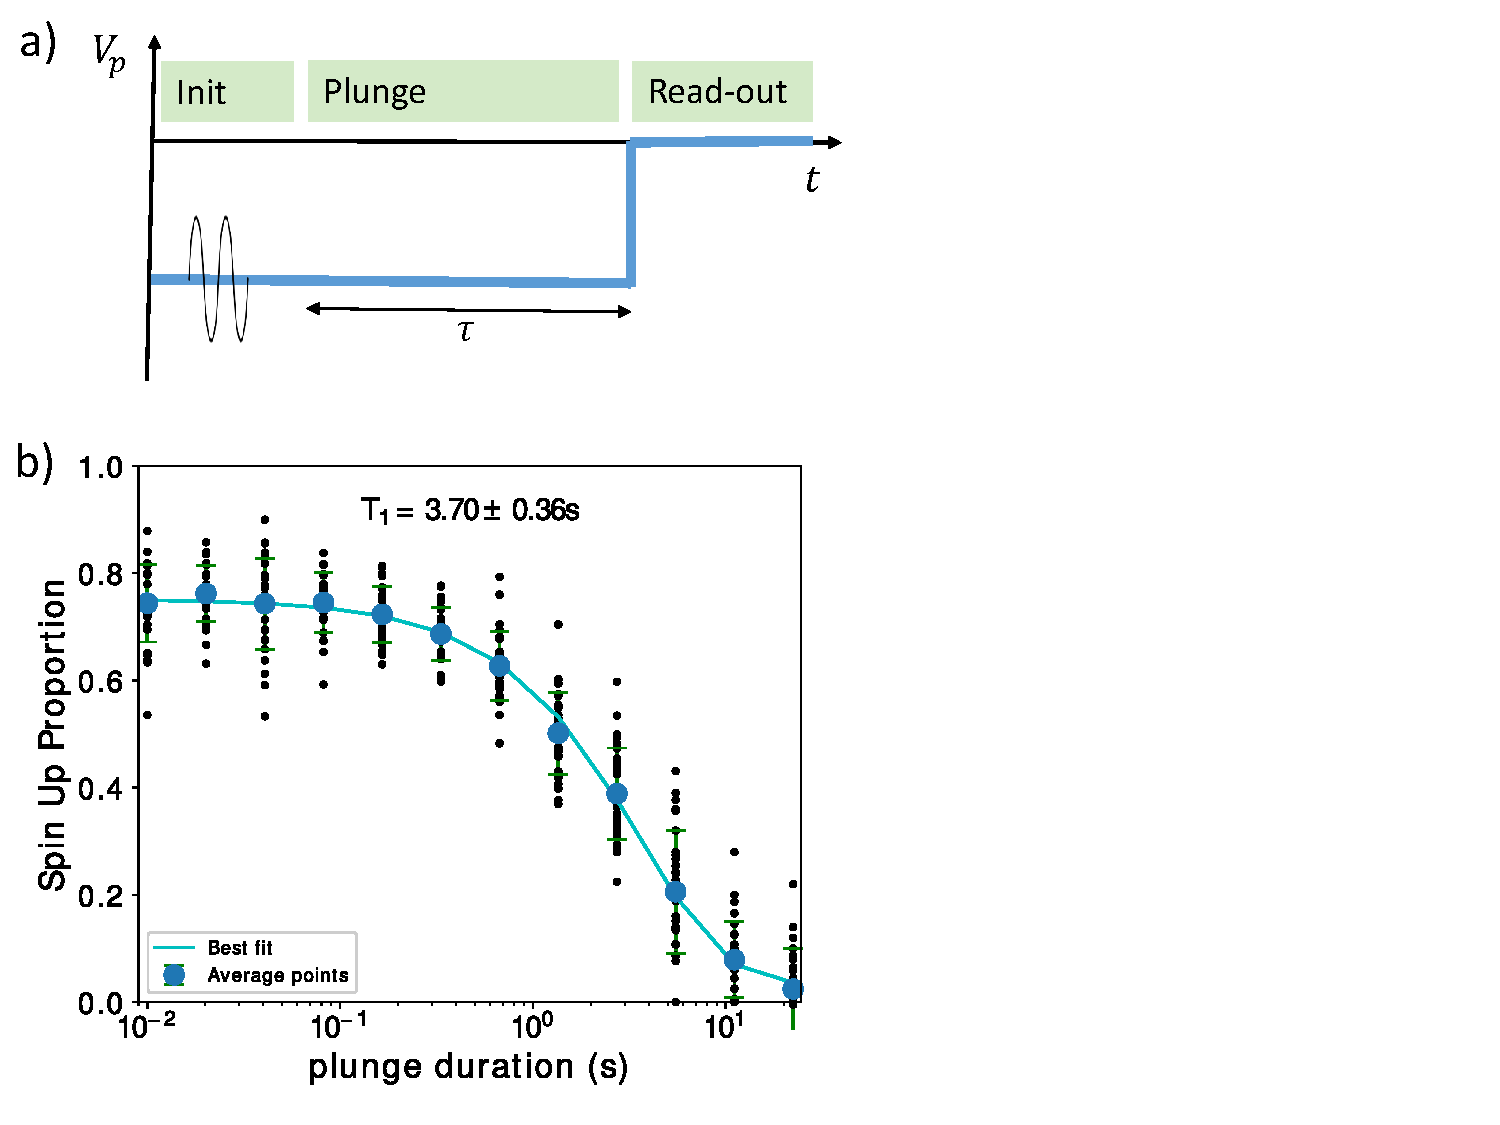
\includegraphics[width=0.7\columnwidth]{figures/fig2.pdf}
\caption{
(a) Schematic of the pulse sequence used in the experiments. The solid line represents the position of the donor energy levels with respect to the Fermi level achieved by the combined voltages of the donor gates. For fields $B_0\leq1.5\,$T, $\ket{\downarrow}$ is initialized and then inverted with an ESR $\pi$-pulse to achieve higher contrast while for $B>1.5\,$T a random load is performed. (b) Example of a $T_1$ measurement at $B=1.5\,$T. For each plunge duration $30$ single shots are taken and averaged to a single point (small black dots). Then the whole measurement is repeated several times and averaged (blue dots) to account for drifts and fluctuations. This uncertainty is expressed through the standard deviation error bars. The relaxation time is extracted by a least-square fit to $T_1=3.7\pm0.4\,$s.
}
\label{fig:t1example}
\end{figure}

To determine the relaxation time $T_1$ of the electron we repeatedly measure the $\ket{\uparrow}$ proportion after a period of time $\tau$ has elapsed while the donor is in the operating regime.  The applied pulse sequence is illustrated in figure \ref{fig:t1example} (a). First, we initialize the electron in $\ket{\downarrow}$ for external magnetic fields of $B_0<1.5$T. Therefore we tune to the readout regime and wait for roughly the tunnel time ($20\,$ms) so that $\ket{\uparrow}$ tunnels into the reservoir and is replaced by $\ket{\downarrow}$. If a high precision is required to increase the measurement contrast, we apply a technique called Bayesian update. A feedback loop is applied that self-corrects for wrongly loaded $\ket{\uparrow}$ and can achieve initialization fidelities of over $99\%$ \citep{Johnson2018}. After $\ket{\downarrow}$ initialization, $\ket{\downarrow}$ is inverted to $\ket{\uparrow}$ by applying an electron spin resonance (ESR) $\pi$-pulse. This concludes the initialization phase. Next, the donor remains for time $\tau$ in the operating regime at plunge depth $V_{p}$. Lastly, a single shot readout is performed in the readout regime. We repeat this sequence $30$ times to acquire one data point of corresponding $\tau$ and then repeat the full measurement multiple times to account for drifts and fluctuations in the electrostatic environment. Figure \ref{fig:t1example} (b) shows an example measurement of the relaxation time at $B_0=1.5$T. The $T_1$ time is extracted by performing a least-square fit. For $B_0>1.5\,$T a random load is performed by simply emptying and reloading an electron, thus preparing either $\ket{\uparrow}$ or $\ket{\downarrow}$ randomly. The remainder of the pulse sequence is the same. The plunge voltage $V_p$ is created by biasing two of the donor gates and the SET top gate simultaneously, changing the electrochemical potential of the donor $\mu_d$ electron with respect to the Fermi level of the SET island. Unless otherwise stated, these pulses are compensated which means that bias of the donor and SET top gate is performed with such a ratio that the SET Fermi level is kept constant while moving the donor. 


\section{Relaxation time dependence on external magnetic field} \label{sec:extB}

\begin{figure}
\centering
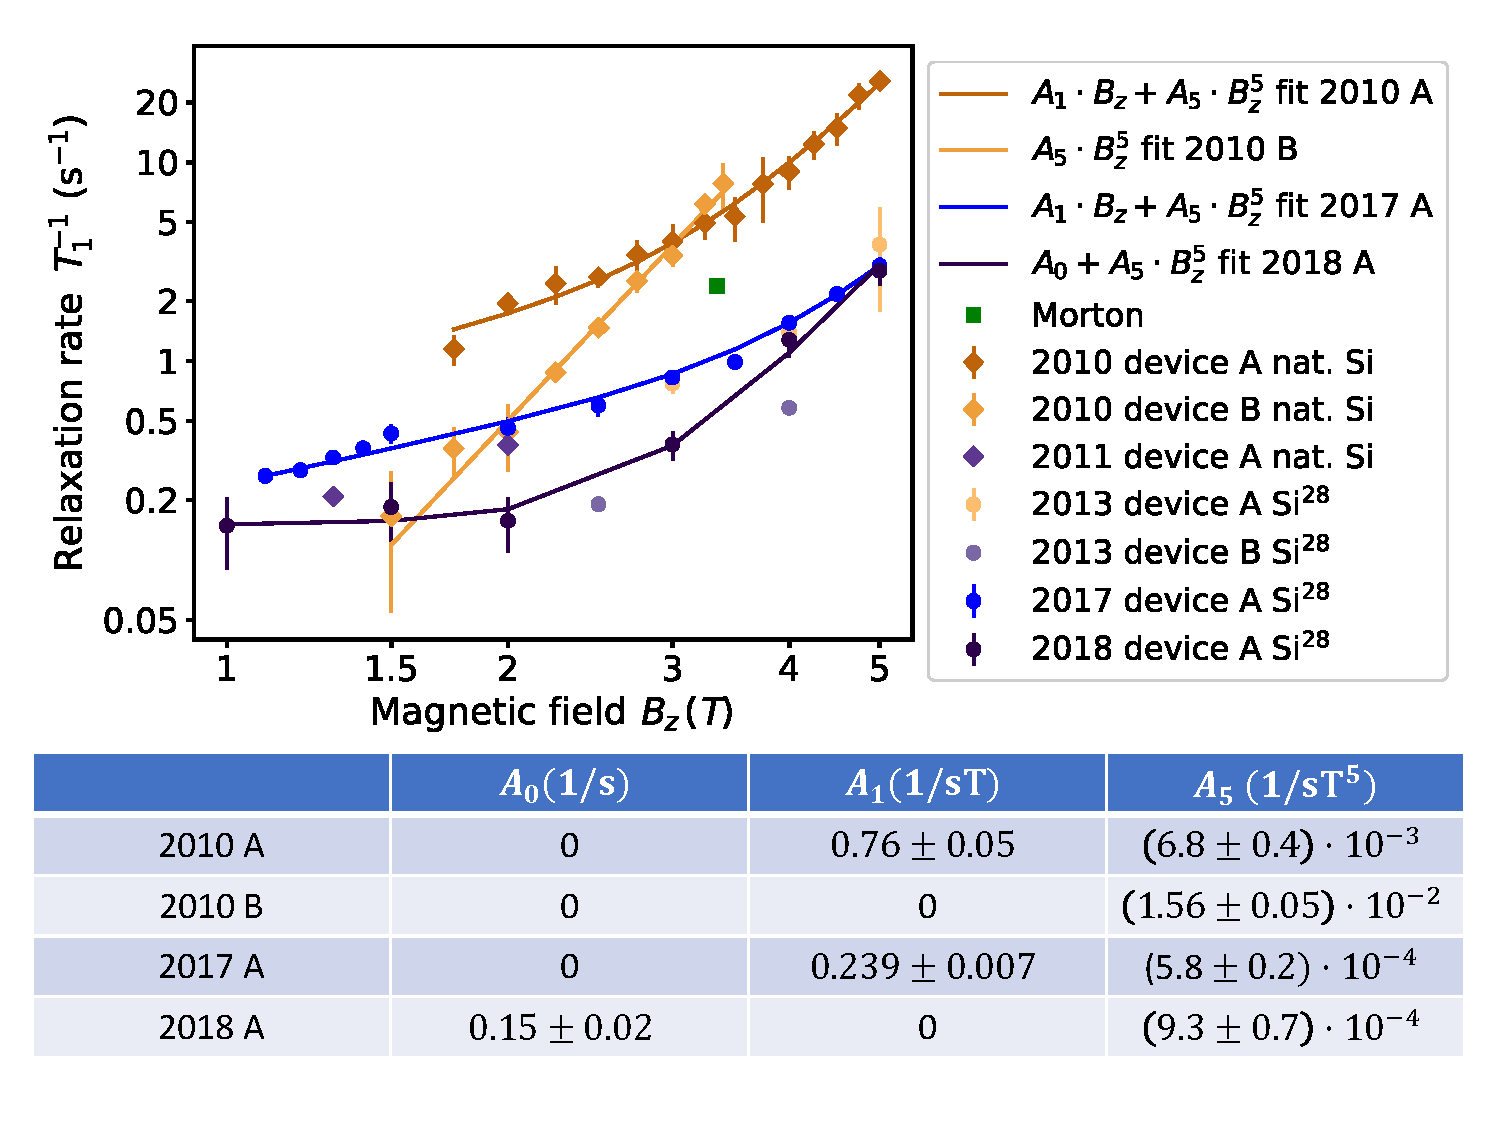
\includegraphics[width=\columnwidth]{figures/fig3.pdf}
\caption{(a) Measurements of the dependence of electron spin-lattice relaxation time $T_1$ on the external magnetic field $B_0$ from different samples. Device 2010A and 2010B are taken from \cite{Morello2010} and are natural silicon, same as device 2011A (squares). Device 2017A and 2018A have been measured on Si$^{28}$, as have devices 2013A and 2013B (dots). For device 2010A, B, 2017A and 2018A curves of form $A_1B_0+A_5B_0^5$ have been fitted. For comparison a measurement of a bulk Si:P crystal at $T<5\,$K is shown (Morton). (b) Fit results of the different samples. 
}
\label{fig:magnetic field dependence}
\end{figure}


In this section we are analysing the dependence of the relaxation time on the strength of the external magnetic field $B_0$. Figure \ref{fig:magnetic field dependence} (a) shows sets of relaxation rates with magnetic field for seven donor qubits with almost identical device layout: devices 2010A and 2010B which are  natural silicon samples, taken from \cite{Morello2010},
device 2011A, also on natural silicon and devices 2013A, 2013B, 2017A, 2018A which are enriched Si$^{28}$ samples. We fit devices 2010A, 2010B, 2017A and 2018A with a polynomial of type $A_0+A_1B_z+A_5B_z^5$ with the results displayed in the table of figure \ref{fig:magnetic field dependence}.  The magnitude of the $B^5$ dependence at high magnetic fields varies significantly between the different devices. This will be explored in section \ref{sec:phonon}.
Furthermore, all fitted devices show a deviation from the expected $T_1\sim B^5$ at magnetic fields below $B_0\approx3\,$T, except for device 2010B. Devices 2010A and 2017A behave as $T_1\sim B_0^1$ while 2018A behaves as $T_1\sim \rm{const.}$. The following section explores an explanation for the $T_1\sim B_0^1$ behaviour.

\subsection{\label{sec:ewjn}Evanescent wave Johnson noise}

\begin{figure}
\centering
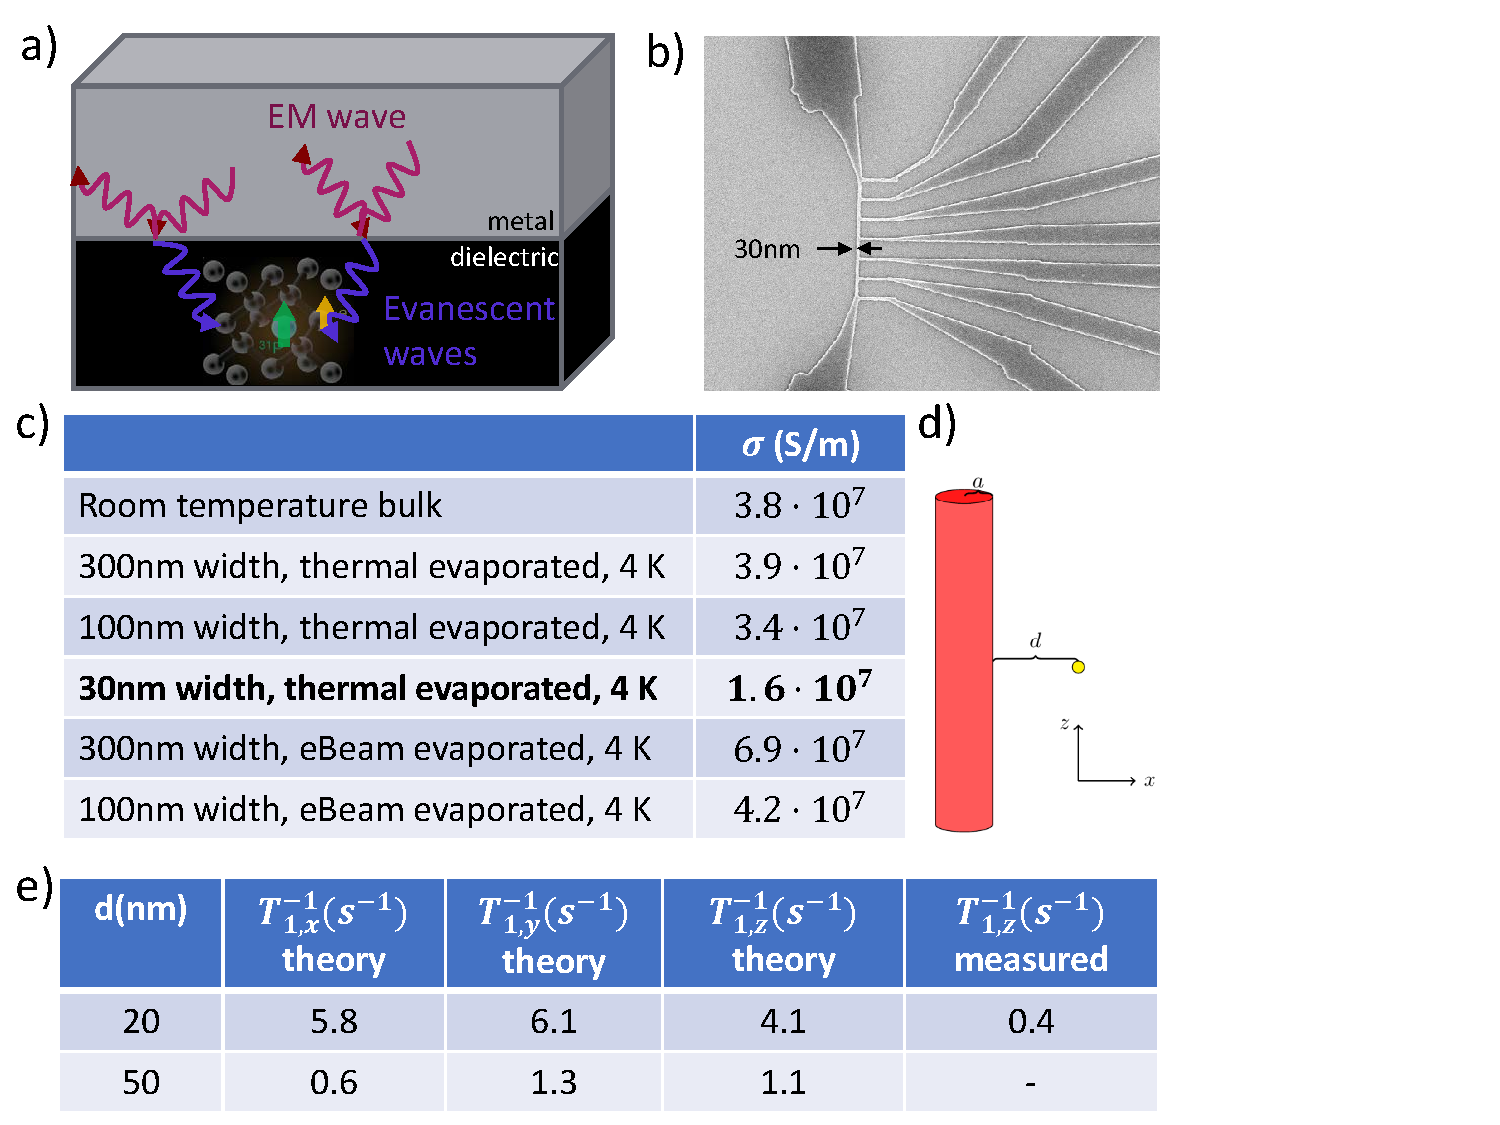
\includegraphics[width=\columnwidth]{figures/fig4.pdf}
\caption{
(a)Schematic of the origin of EWJN in our qubit devices. (b) Scanning electron micrograph of a Hall bar structure with feature size of $30\,$nm. (c) Table of conductance values of Aluminium, measured with  Hall bar structures as in (b), for different feature sizes and evaporation techniques. Aluminium thickness is 50nm. Room temperature bulk value for comparison \cite{Serway1998}. (d) Geometry assumption for theoretical EWJN calculations where the cylinder represents the metal gate on top of the qubit (small yellow circle) with diameter $a$ and distance $d$. (e) Table of relaxation rates predicted by the EWJN theory and measured value at $B_0=1.5\,$T. 
}
\label{fig:ewjn}
\end{figure}

Our qubits are in the vicinity of metal electrodes that contain mobile charges and spins. The thermal and quantum motion of these creates random electromagnetic fields that decohere and relax the qubit. This we know as Johnson noise \cite{Johnson1928, Nyquist1928, Callen1951}. It leaks out of the metal into the insulator in form of evanescent waves when the photons are reflected on the metal-insulator interface as depicted in figure \ref{fig:ewjn}. Thus there is strong Johnson noise near the metallic surface which is called evanescent wave Johnson noise (EWJN) \cite{Henkel1999, Poudel2013, Premakumar2017}. At low temperatures this can lead to relaxation as the evanescent waves create many available photon states which enhances spontaneous emission for the donor electron. For this type of magnetic noise that couples directly to the electron spin, we can write for $k_BT\ll g_0\mu_B B_0$ the relaxation rate as

\begin{equation}
T_1^{-1}=\frac{1}{\mathcal{L}}\frac{\mu_B^2\sigma\omega_0}{\hbar c^2}
\end{equation}

where $\mathcal{L}$ is a geometric factor that depends on the geometry of the device, $\sigma$ is the conductivity of the metal structures, $\omega_0$ is the Larmor frequency of the qubit which depends on the magnetic field $\omega_0=\frac{g_0\mu_B B_0}{\hbar}$. $g_0$ is the electron g-factor, $\hbar$ the reduced Plank constant, $c$ the speed of light in vacuum and $\mu_B$ the Bohr magneton. Thus the relaxation follows $T_1^{-1}\sim B_0$. This theory anticipates a local response. Consequently the skin depth $\delta=1/\sqrt{\mu_0\mu_R\sigma\omega_0/2}$ has to be large compared with the dimensions of the metallic elements of the device and the distance of the qubit from those objects. Furthermore, the conduction in the electrodes has to be in the diffusive regime where the mean free path $l_F=v_F\frac{m_e}{ne^2}\sigma$ ($v_F$ is the electron Fermi velocity, $m_e$ the electron mass, and $n$ the electron density) is much shorter than the device dimensions.  

As the conductance of the aluminium structures directly relates to both the validity of the model through the characteristic length scales and the resulting magnitude of the relaxation, we carefully measure it with 4-point measurements on Hall bar structures with feature sizes varying from $300\,$nm to $30\,$nm for both thermal and electron beam physical vapour deposition (EBPVD). Figure \ref{fig:ewjn} (b) shows a scanning electron micrograph of a $30\,$nm Hall bar device while table \ref{fig:ewjn} (c) shows the resulting conductance values for all measured structures. 
We find that the conductivity drops with reduced feature size but only up to a factor of 2 which is conclusive with our feature size of approximately $20\,$nm.  We choose the $30\,$nm thermal measurement $\sigma=1.6\cdot 10^7\,$S/m for further calculations as this resembles most closely the qubit device measured in this paper. This results in a skin depth of $\delta=752\,$nm and mean free path of $l_F=19\,$nm. Thus, while the skin depth is sufficiently large, the mean free path is comparable with our feature size of around 30nm. This means that we are on the brink between the ballistic and diffusive regime which might reduce the EWJN.

We calculated the geometric dependence according to our device geometry by assuming a conducting cylinder of diameter $a$ and distance $d$ from the qubit as shown in figure \ref{fig:ewjn} (d). In our case $d$ and $a$ are of similar magnitude. Thus we employ an interpolation between the qubit seeing a half-space sphere ($d\rightarrow 0$) and the qubit being far away ($d\gg a$) which predicts the relaxation rate to 
\begin{subequations}
\begin{equation}
T_{1,x}^{-1}=\frac{\mu_B^2\sigma\omega_0}{\hbar c^2d}\frac{\frac{75\pi^2}{1024}\frac{a^4}{d^4}\frac{3\pi}{4}}{\frac{75\pi^2}{1024}\frac{a^4}{d^4}+\frac{3\pi}{4}}
\end{equation}
\begin{equation}
T_{1,y}^{-1}=\frac{\mu_B^2\sigma\omega_0}{\hbar c^2d}\frac{\frac{273\pi^2}{1024}\frac{a^4}{d^4}\frac{3\pi}{4}}{\frac{273\pi^2}{1024}\frac{a^4}{d^4}+\frac{3\pi}{4}}
\end{equation}
\begin{equation}
T_{1,z}^{-1}=\frac{\mu_B^2\sigma\omega_0}{\hbar c^2d}\frac{\frac{147\pi^2}{512}\frac{a^4}{d^4}\frac{\pi}{2}}{\frac{147\pi^2}{512}\frac{a^4}{d^4}+\frac{\pi}{2}}
\end{equation}
\end{subequations}

With our experimental parameters, EWJN predicts relaxation rates of $T_1\approx5\,\rm{s}^{-1}$ as shown in table \ref{fig:ewjn} (e). We find our theory to agree well with our measurement of device 2013A while it overestimates the relaxation rate by around one order of magnitude for device 2017A. We have to keep in mind though that the donor depth is uncertain within $\pm10\,$nm due to the implantation process \cite{VanDonkelaar2015}, as well as the exact donor position with regard to the metal gates. This can account for variations between different devices, even though the same metal gate structure was used. Nevertheless a donor depth much beyond $20-,$nm seems unreasonable, given that we are able to easily readout the donor with our SET. Thus the theory indeed seems to overstate the EWJN relaxation. This is quite puzzling. One explanation could be that ballistic effects reduce the EWJN. Additionally, the interpolation formula seems to be favouring the near-limit, thus potentially overestimating the relaxation rate. 

Another interesting fact is that neither device 2010B nor device 2018A does exhibit this behaviour within the measured range. This might be due to a donor position further away from the metal gates or deconstructive interference. %though this seems unlikely for several magnetic fields?
The constant offset device 2018A shows at low magnetic field may be explained by the presence of Si$^{29}$, which have been observed to interfere with the qubit, even in purified silicon devices\cite{Morello2010}. 

\subsection{\label{sec:phonon} Strain enhanced phonon induced relaxation}

Figure \ref{fig:magnetic field dependence} shows a striking difference in magnitude of the phonon induced $T_1\sim B^5$ relaxation. The devices show a different relaxation coefficient of up to two orders of magnitude. 

We relate this to different amounts of strain in the various devices. Strain arises due to the different lattice constant of Aluminium and silicon \cite{Thorbeck}. As our donors are quite close to the Aluminium silicon interface, their environment will see significant strain. This has been observed in previous measurements\cite{Laucht2015, Asaad2018}. 
Eq. \ref{eq:fullT1} shows that the phonon induced relaxation depends on the valley-orbit splitting $E_{12}$. The splitting reduces with strain as the donor orbital becomes slightly more dot-like \cite{Tahan2002} which in turn reduces $T_1$. However, strain also reduces the phonon matrix transition element between the ground and first excited state dramatically which greatly increases $T_1$. The latter was found to be the dominant effect by Tahan \textit{et. al.} \cite{Tahan2002}.  
 
We know that device 2017A is fairly strained with $s_{xy}=-0.1\%$ in-plane compressive strain, estimated by atomic tight binding simulations by Laucht \textit{et. al.} \cite{Laucht2015}. Device 2018A has a hyperfine interaction constant of $A=115\,$MHz, which corresponds to a strain of $s_{xy}=-0.05$. Furthermore, the relaxation of device 2010B exactly coincides with the relaxation measured in a STM hydrogen lithography device by \cite{Watson2015}. The STM device is assumed strain less as there are no metal gates anywhere close to the donor. We speculate that device 2010B was a deep donor, relatively far away from the Aluminium gates. This would also explain the lack of EWJN. 
Overall, this observations confirm the trend that strain increased the phonon-induced relaxation time. 


\section{\label{sec:cotunnelling} Tunnelling effects}

To analyse the dependence of the relaxation time on the electrostatic environment we start by measuring the relaxation at different donor plunge voltages. The plunge voltage depth and direction with respect to the Fermi level determine how far the donor electron spin states are confined below the Fermi level. 
Usually, for electrons to be able to tunnel between the donor and the SET, they have to conserve energy. However, due to the Heisenberg uncertainty principle, energy conservation can be broken for a time $t_H\approx\frac{\hbar}{E_c}$, where $E_c$ is the confinement of the electron. In this time frame, tunnel effects can appear which relax the donor spin. First order tunnelling (direct tunnelling) is described by 

\begin{equation}\label{eq:directt}
\Gamma_{\rm DT} = \Gamma_0\cdot f(E, T)
\end{equation}
with the Fermi function $f(E,T)=1/(\left(1+e^{-{e\alpha V_p}/{k_B T}}\right)$. $\Gamma_0$ is the tunnelling rate from the donor to the SET island when the energy of donor is aligned with SET Fermi level, $\alpha$ is the lever arm of the gate voltages to the qubit and $T$ is the electron temperature of the SET electron reservoir \cite{Golovach2004, MacLean2007}. This tunnel process is exponentially suppressed with the donor distance to the Fermi level and is only expected as long as at least one donor spin state is at or above the Fermi level. 

Second order tunnelling (co-tunnelling) is described by 

\begin{equation}\label{eq:cot}
\Gamma_{\rm CT} = \frac{\hbar}{\pi}\Gamma_0^2\frac{E_z}{\left(e\alpha V_p\right)^2}
\end{equation}
with $E_z=g_0\mu_B B_0$ as the Zeeman energy \cite{Quassemi2009, Lai2011, Otsuka2016}. This tunnel process is also suppressed with donor distance but less strongly and remains possible way below the Fermi level. However for a low direct tunnel rate $\Gamma_0$ this process is quite unlikely. 

\begin{figure}
\centering
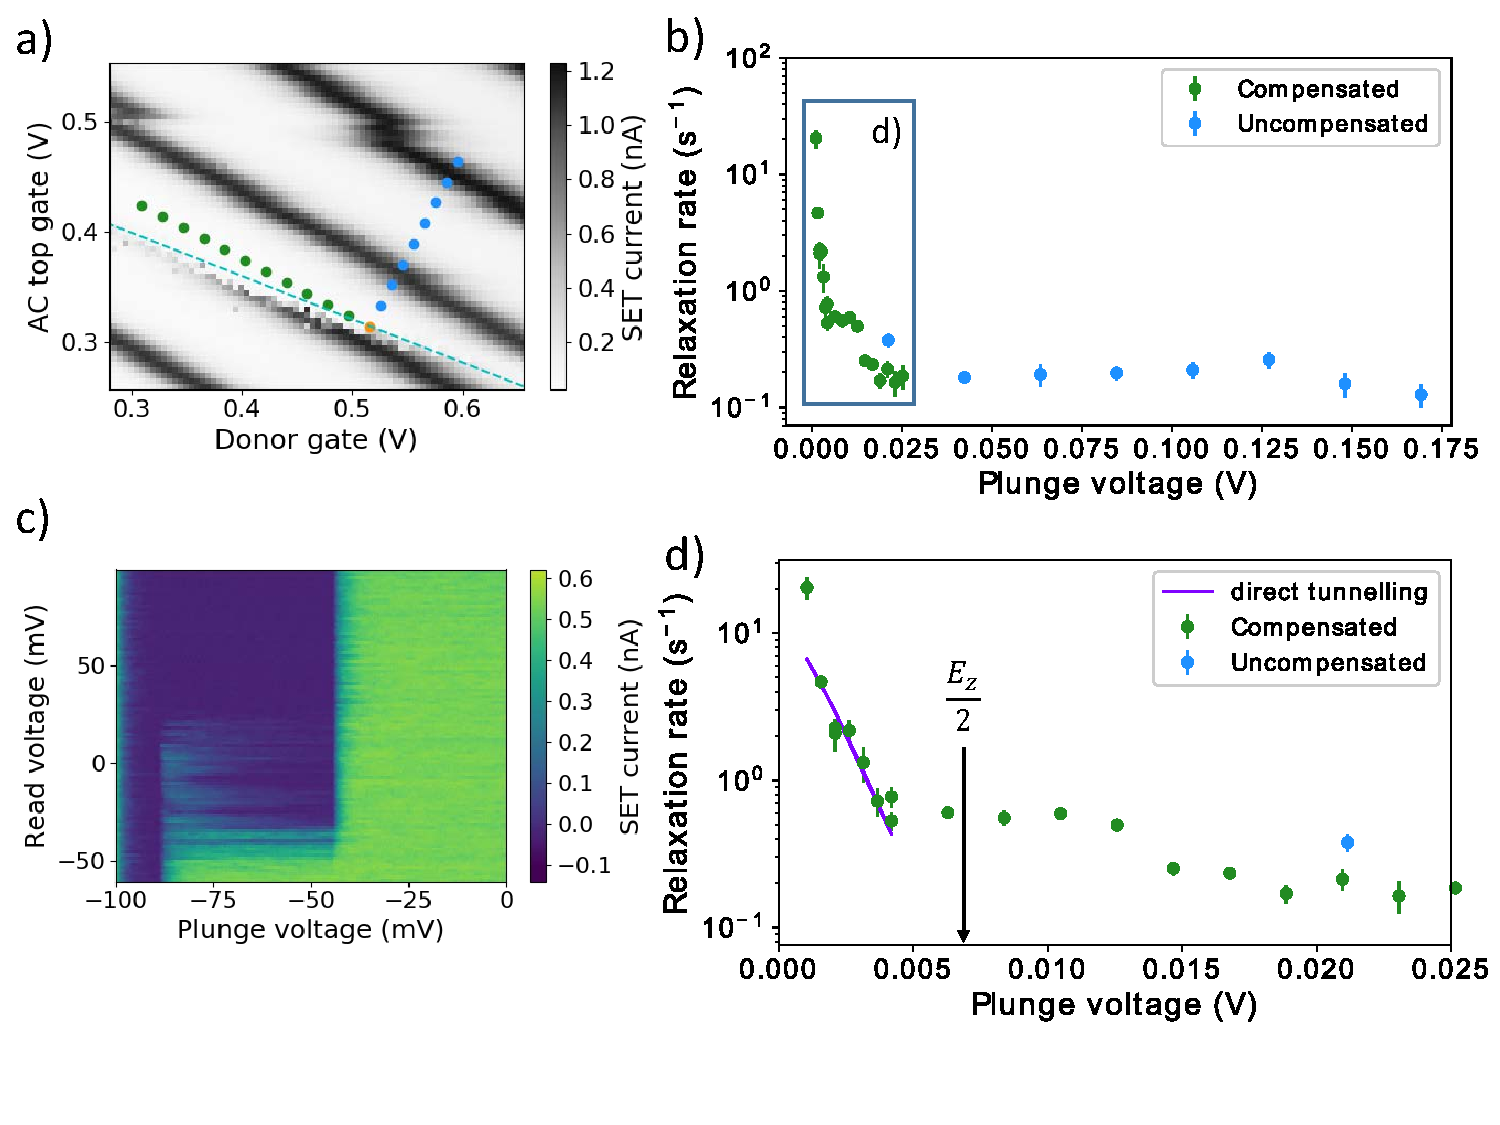
\includegraphics[width=\columnwidth]{figures/fig5.pdf}
\caption{
(a) Charge stability diagram with the donor charge transition indicated in dotted blue. The green points represent the compensated plunging, where the SET Fermi level is kept constant while the donor is moved. The blue points are uncompensated plunging so that we can achieve deeper confinement in the plunge stage. (b) Relaxation rates with plunge voltages, both uncompensated and compensated. The uncompensated plunge voltage represents the geometric distance to the donor transition - this is only the approximate distance to the Fermi level (dotted blue in (a)). The square indicates the region we show in greater detail in (d). (c) Read level voltage varied with plunge voltage to determine the Zeeman splitting through the spin tail. (d) Zoomed-in plot for low plunge voltages with Zeeman energy $E_z$ marked. The direct tunnelling has been fitted with an exponential. 
}
\label{fig:plungedependence}
\end{figure}

In figure \ref{fig:plungedependence} we present the measurements of the relaxation time for different donor plunge depths. Figure \ref{fig:plungedependence} a) shows the measured donor plunge points with respect to the SET Fermi level (blue dotted line) in the charge stability diagram. We both measure along the direction of the Coulomb peaks of the SET, keeping the SET Fermi level constant (compensated plunging, green points), as well as perpendicular to it, achieving very deep plunge amplitudes (uncompensated plunging blue points). In figure \ref{fig:plungedependence} b) the corresponding relaxation rates are plotted where the plunge voltages are normalized to the geometric distance to the Fermi level. For the uncompensated measurements this serves only as an approximation of the distance to the Fermi level which moves a different amount for each uncompensated plunge value. 
As expected, the relaxation rate strongly decreases the deeper the donor is plunged below the Fermi level until it stabilises at around $T_1^{-1}=10^{-1}\,$s$^{-1}$. Clearly we identify two regimes: On the one hand, at high plunge voltages ($V_p>20\,$mV) the relaxation remains constant which implies that the relaxation rate is not limited by any type of tunnel process. On the other hand, at low plunge voltages we observe a strong dependence. Hence figure \ref{fig:plungedependence} (d) shows a zoom on plunge voltages between $0\,$V and $25\,$mV. 
To compare the energy scales we determine the lever arm between the compensated plunge voltage and the donor energy. Therefore we measure the SET current while varying the donor read voltage level from a position where both spin states are above the Fermi level, causing a high current by conduction through $\ket{\downarrow}$, to a position where both donor states are below the Fermi level, blocking conduction fully. In the intermediate regime where just $\ket{\uparrow}$ is above the Fermi level we see a so called spin tail when the up-electron tunnels out and is replaced by a spin down electron. The length of this spin tail corresponds to the Zeeman energy at the applied external magnetic field. Figure \ref{fig:plungedependence} (c) shows a spin tail measurement at $B_0=5\,$T. We calculate the lever arm to $\alpha=8.3\cdot 10^{-3}$ and $V_p^{Z}(B_0=1\,\rm{T})=14\,$mV. At $V_p=0$ the donor is tuned such that the Fermi level is half way between $\ket{\uparrow}$ and $\ket{\downarrow}$. Consequently, both donor states will move below the Fermi level at the voltage corresponding to half the Zeeman energy, marked in figure \ref{fig:plungedependence} (d). Within this small region, we again can clearly identify two regimes: For $V_p=[0,5]\,$mV where we see an exponential dependence due to direct tunnelling from $\ket{\uparrow}$ to the SET reservoir limiting our relaxation. We fit Eq. \eqref{eq:directt} to the data points and find $\Gamma_0=18\pm5\,$Hz which agrees well with the standard tunnelling times we observe in our readout traces of tens of ms. 


\begin{figure}
\centering
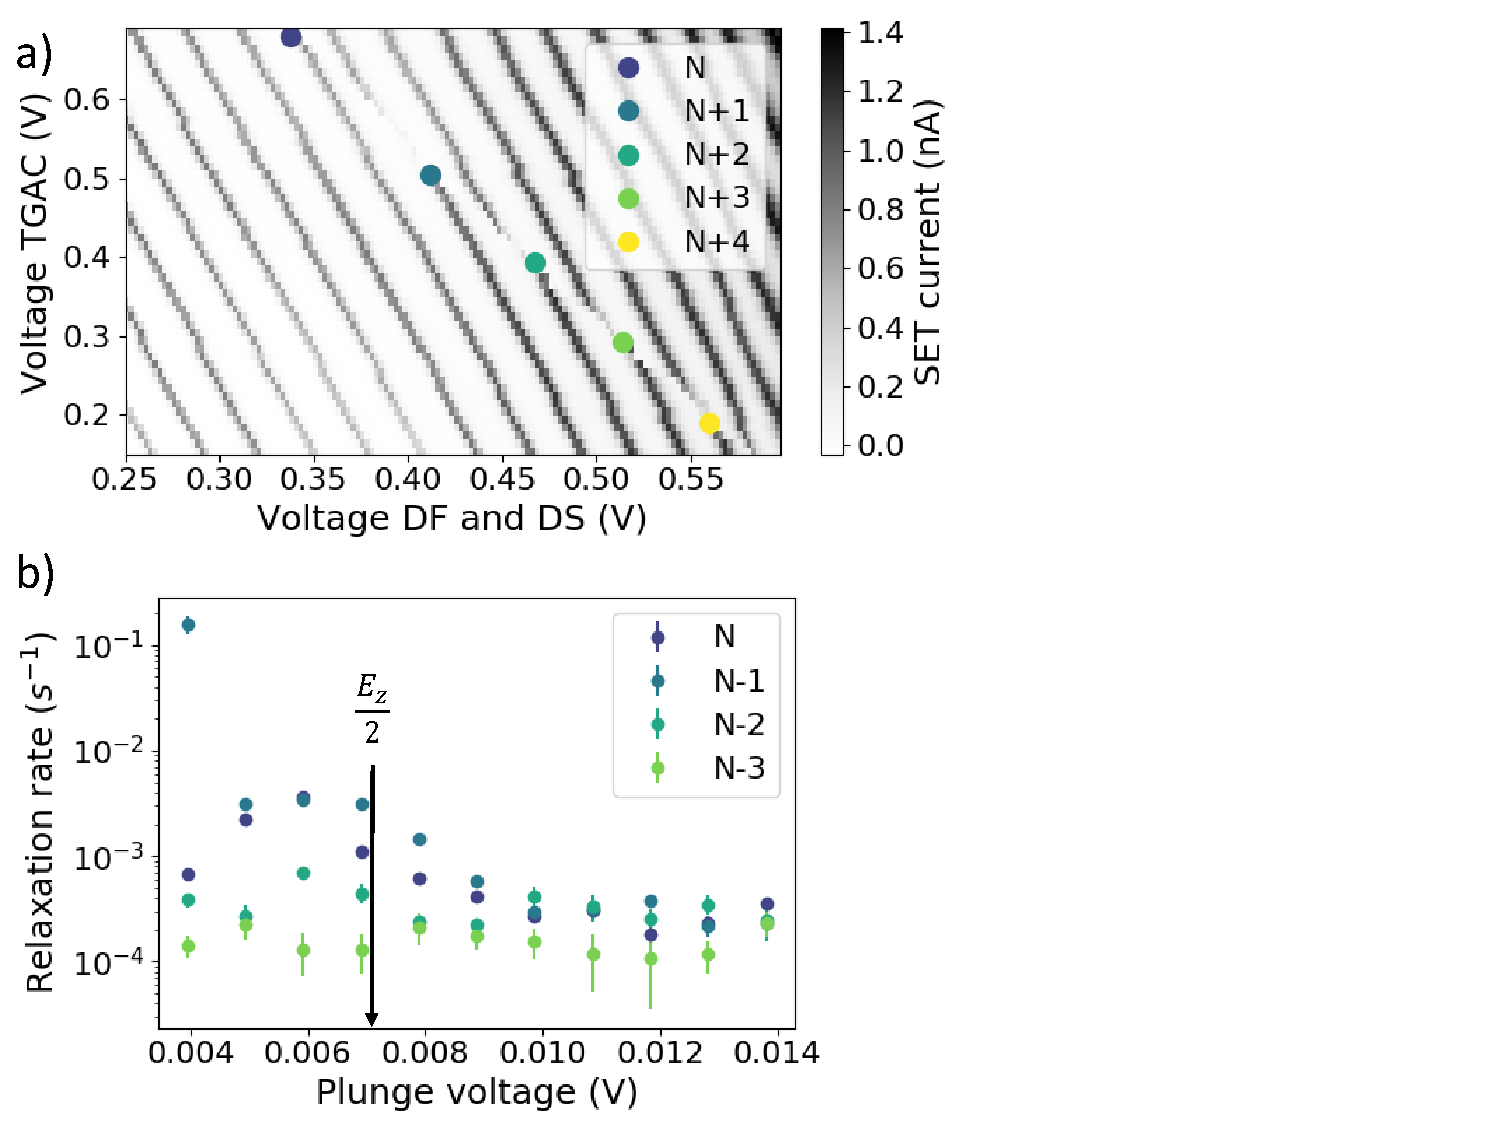
\includegraphics[width=0.8\columnwidth]{figures/fig6.pdf}
\caption{
(a) Charge stability diagram with measurement points for different SET island electron number indicated. (b) Relaxation rates with plunge voltage for different SET island electron numbers while plunging compensated. 
}
\label{fig:electronnumberdependence}
\end{figure}

To further confirm this results we measured the relaxation time for several different Coulomb peaks of the SET which means that the electron number of the SET island varies.
Figure \ref{fig:electronnumberdependence} (a) shows the measurement points on the charge stability diagram while figure \ref{fig:electronnumberdependence} (b) shows the corresponding relaxation times with plunge dependence. We operate our SET in the semi-classical regime with around 100 electrons, where the Fermi distribution is basically continuous but its shape still depends on the number of electrons. As the tunnel rates depend on the density of states of the SET island reservoir, they vary with electron number. Thus, at low plunge voltages we observe significant differences in the relaxation rates while for deep plunging these differences disappear as the tunnel processes are suppressed. 


\section{\label{sec:conclusion}Conclusion}

In summary, we find that EWJN is a likely candidate for the reduction of the relaxation time at low magnetic fields if the qubit is close to a strongly conducting surface, like metallic gates. Moreover, we discover that strain at the donor site has the opposite effect and increases the relaxation time. This can indeed lead to very long $T_1$ times such as 10s. Furthermore, tunnel effects increase relaxation if one does not confine the donor electron strong enough. 

Overall, we believe that this work gives many new insights in the fundamental physics of donors in silicon which will help engineer our qubits to perform even better.  





